\subsection{Job Interviews \& Job Application Videos}
Many organizations and corporations use job interviews to select the most qualified person for an open position. Job interviews typically consist of a short meeting where the applicant is assessed based on their skills and experience but also on their personality, mood, energy and motivation during the interview. A study by Kraus and Kurtis (\citeyear{kraus1990creative}) shows that managers also base their decision heavily on their overall impression of the applicant. These dimensions are assessed to determine and predict if the applicant would be successful at the job they have applied for. Hiring an incompetent worker would not only mean the loss of salary but also the time it takes to search for a new candidate. A study by Dettmar (\citeyear{dettmar2004we}) shows that these implicit and explicit costs of hiring the wrong candidate combined could be as much as that of a years salary of that new hired worker. Despite this risk, job interviews prove to be a reliable method in the job candidate selection process (\cite{weekley1987reliability}). 

However, with the increase in use of online communication tools and online application processes job the approach for job interviews has changed as well. Many organizations choose to use online platforms to recruit new employees for open positions. A study in 2011 showed that 76\% of unemployed people search online for new jobs (\cite{faberman2016does}), which is an indication of how reliant organizations have become on online job recruitment. Research has been done to improve the online recruitment process by increasing market transparency and lower transaction cost with the use of semantic web technologies (\cite{bizer2005impact}). Further, video resumes have become increasingly popular as a result of the increase of use of online communication platforms. Studies show that video resumes are mostly made by a young demographic who are looking for a junior position (\cite{nguyen2016hirability}). In addition to online video resumes, a new type of online job interviewing has also emerged which is called asynchronous video interviews (\cite{torres2017asynchronous}). This type of interviewing involves an applicant who sends a video recording of them answering interview questions (\cite{toldi2011jobapplicants}). On the other hand, synchronous video interviewing are held on platforms like Skype, Microsoft Teams and other video conference software. These new methods of interviewing can decrease costs as they prove to be more time-efficient (\cite{weber2012your}).

\subsection{Personality Traits}
The assessment of personality traits is equally important when analyzing and determining which candidate is the most suitable for the position (\cite{kinsman2005hiring}). However, assessing a person's personality can be a rather difficult task. Therefore, we must first understand how personality is defined and how to analyze it. 

In psychology, the characterization of someone's personality is based on long-term behavior. Personalities have sophisticated structures and are constructed of many different aspects such as habits and the way people think or feel. Therefore, it can be difficult to analyze, measure and categories personalities to divide humans into different personality types. Instead, psychology now mainly focuses on personality traits, where the OCEAN (or CANOE) Big Five personality trait model developed by Paul Costa and Robert R. McCrae (\cite{costa1992neo}) is most widely accepted. These traits are; Openness to experience, Conscientiousness, Extraversion, Agreeableness and lastly, Neuroticism. 

The first factor of the 5 factor personality trait model is Openness to experience. People who score high in this factor generally are imaginative and care more about aesthetics, ideas and values (\cite{mccrae1993openness}). The Conscientiousness factor is related to how well-organized and persistent a person is. People with high conscientiousness are considered caring, dependable and organized (\cite{widiger2017oxford}). The traits underlying the Extraversion dimension are related to sociability and activity. Extraverted people are more talkative, adventurous and sociable while introverted people tend to be more silent, cautious and focused on their inner state of mind(\cite{widiger2017oxford}). Agreeableness is a dimension of interpersonal behavior. People with high scores on agreeableness are cooperative, good natured and are seen as friendly (\cite{graziano1997agreeableness}). Lastly, the Neuroticism dimension represents a person's tendency to experience emotional anxiety (\cite{widiger2017oxford}). The dimension can also be described as someone's emotional stability. People with high neuroticism are more anxious and nervous and tend to worry more while people with low scores are more calm and composed. 

Several works have used the five factor personality model to analyze human behavior. \textcite{quercia2011our} for example, who analyzed relationships with different types of Twitter users. They were able to predict the personality types of Twitters users based on their following, followers and listed counts.  Further, \textcite{allbeck2008creating} used the OCEAN model to map personalities to crowd simulations in order to improve the realism of their simulations. They used the OCEAN model as a basis for their simulation agents of psychology. The resulting simulations has shown the impact of different personality traits in crowds. 

\subsection{Apparent Personality Analysis}

Another approach to apply the five factor model is to analyze and annotate the apparent personality traits (\cite{junior2018first}, \cite{chen2016overcoming}), rather than the actual personality traits. In this process, an annotator annotates the impression a subject leaves rather than the actual personality. This is easier as the annotator relies on external evaluations without any direct involvement of the subject. 

Several studies have shown that the modeling of apparent personality traits is possible from different modalities like text (\cite{gievska2014impact}, \cite{alam2013personality}), speech (\cite{valente2012annotation}, \cite{madzlan2014towards}) and also video based (\cite{junior2018first}, \cite{qin2016modern}, \cite{escalante2020modeling}). On top of that, research has been done on modeling job interview decisions based on apparent personality traits from different modalities, including the video based modality (\cite{kaya2017multi}, \cite{kaya2018multimodal}, \cite{yu2019multimodal}). These papers prove that the modeling of apparent personality traits is feasible and show high scores in classification accuracy. 

Further, deep learning based classifiers are used in this thesis to model apparent personality traits and other dimensions. Compared to other methods of feature extraction, deep learning is becoming more widely used as it proves to be more robust. For example, it has been applied in the recognition of faces (\cite{parkhi2015deep}), emotion recognition (\cite{kaya2017video}) and modeling job interview decisions (\cite{kaya2018multimodal}). 

\subsection{Mood Primitives \& Likeability}
Another dimension that can be used to classify a person's behavior is to assess their mood or emotions over a short period of time. While the terms emotion and mood seem to be used interchangeably, they are in fact different. In psychology, an emotion is seen as a immediate reaction to a stimulus, while a mood lasts for a longer period (\cite{bower2000affectmemory}). For example, someone can be in positive mood throughout the day but still have a negative emotional reaction to a stimulus like a bad smell, or being insulted (\cite{matlin2012cognition}). Additionally, this makes it more difficult to identify and specify the cause of someone's mood as there is no direct cause like in a emotional reaction (\cite{desmet2016mood}).

In order to simplify the classification of a subject's mood, emotion classification can be used. Instead of trying to determine someone's mood over a short period, the emotions can be used as an indicator or their mood. To do this, a base set of emotions is needed to start classifying a subject's mood. The six basic emotions developed by Paul Ekman in 1992 are widely regarded as the standard to identify emotions (\cite{ekman1992argument}). Figure \ref{fig:basicemotion} illustrates the emotions as described by Ekman. Ekman found that there are nine distinct characteristics that distinguish the basic emotions, for example, the physiological response, the duration and their quick onset. He also found that cultural background had no impact in the identification of emotion. Meaning that the six basic emotions can be used across different cultures to classify emotions. The six emotions that Ekman identified as basic are; anger, happiness, surprise, disgust, sadness and fear (\cite{ekman1992argument}). 

\begin{figure}[h]
  \centering
  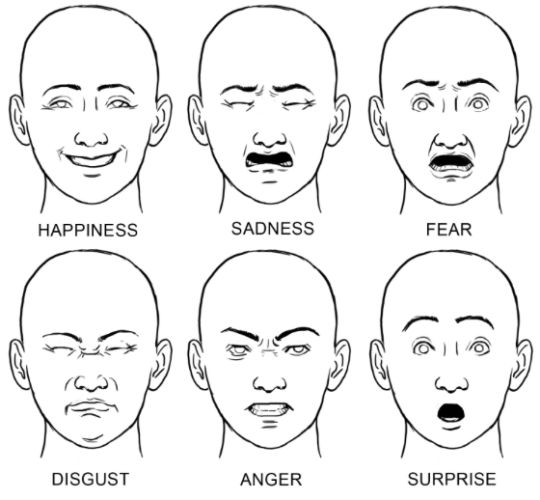
\includegraphics[width=\columnwidth]{Images/ekman_six_emotion.png}
  \caption{The 6 basic emotions as proposed by Ekman.}
  \label{fig:basicemotion}
\end{figure}

Research has also indicated that mood can be defined as a dimensional model with two dimensions: valence and arousal. This model was first proposed by Russel in 1980 (\cite{russell1980circumplex}), and is known as the circumplex model of affect. In this model arousal can be seen as the amount of energy a person shows. This dimension ranges from a deactivated state, described as sleepiness, to an activated state, which can be described as aroused. The valence dimension refers to the pleasantness or unpleasantness. This dimension typically ranges from a state of misery to a state of pleasure. Combining these two dimension creates four quadrants with four basic moods; angry, happy, sad and relaxed. Figure \ref{fig:circumplexrussel} shows the circumplex model and indicates where the basic moods would be positioned on this model.

\begin{figure}[h]
  \centering
  \includesvg[width=\columnwidth]{Images/russell_dimensions.svg}
  \caption{The circumplex model of affect as proposed by Russel.}
  \label{fig:circumplexrussel}
\end{figure}

The dimensional model has been used by \textcite{desmet2016mood} to develop a method that can be used to identify moods. In their paper, \citeauthor{desmet2016mood} propose a pictorial scale to report or express a mood. The pictorial scale consists of eight different moods, two for each quadrant on the circumplex model. However, in this thesis, the valence and arousal dimensions will be regarded as two separate dimensions which will be annotated with an ordinal scale as opposed to having a single categorical mood dimension.

Another dimension that can be modeled to automate the job candidate screening process is likeability (\cite{celiktutan2015automatic}). Likeability usually refers to whether someone is seen as friendly and social. Although likeability is a highly subjective dimension, research has shown that it is associated with the Big Five personality traits of extraversion and neuroticism, while being positively related to agreeableness (\cite{van2010classroom}). Studies have also shown that likeability is a significant factor in the hiring processes (\cite{raza1987model}). \citeauthor{hayes1997comparison} (\citeyear{hayes1997comparison}) also found that an applicant's attractiveness has an effect on the likeability of the applicant. However, little research has been done on using video features to model the likeability of an applicant and predict whether an applicant should be invited for a job interview. This will be explored further in this thesis. 
